\documentclass{article}

\usepackage[normalem]{ulem}
\usepackage{fancyhdr}
\usepackage[parfill]{parskip}
\usepackage{tikz}
\usepackage{pgfplots}
\usepackage{multicol}
\usepackage[version=3]{mhchem}
\usepackage{SIunits}
\pagestyle{fancyplain}

\pgfplotsset{compat=1.7}

\title{Nuclear Physics}
\author{Todd Davies}
\date{\today}

\begin{document}

\rhead{Nuclear Physics}
\lhead{\today}

\maketitle

\section*{Nuclear fission}
\thispagestyle{empty}

Nuclear fission occurs when a large and unstable nucleus splits into two smaller
nuclei and some neutrons. This happens when a neutron hits the large and
unstable nucleus. The neutrons that are released will fission another unstable
nucleus if they hit it, which fuels more fission.

This is what happens in nuclear power plants, and it releases energy.

We can represent fission reactions by equations such as this:
\marginpar{Note the number of protons and neutrons are constant in the reaction}

\[
	^{1}_{0}n + ^{235}_{92}U \rightarrow 
	^{92}_{36}Kr + ^{141}_{56}Ba + 3^{1}_{0}n
\]

There are intermediate reactions in these reactions too since the large unstable
nucleus probably won't decay into two other nuclei straight away, but rather
accept the incoming neutron and then decay:

\[
	^{1}_{0}n + ^{235}_{92}U \rightarrow 
	^{236}_{92}U^{*} \rightarrow
	^{92}_{36}Kr + ^{141}_{56}Ba + 3^{1}_{0}n
\]

\section*{Energy release in fission}

The measured mass of any nucleus is less than the mass of it's consitiuent
particles. This 'loss' of mass is known as the {\it mass defect} of an atom, and
it is linked to the {\it binding energy} of the nucleus.

The binding energy is the minimum energy needed to seperate all of the protons
and neutrons in the nucleus and we can use $E = MC^2$ to work it out.

%TODO:Verify this...

The change in the binding energy between the reactant nucleus of the fission
reaction and the products of the fission reaction results in the release of
energy.

\section*{Binding energy and stability}

The higher the binding energy of the nucleus, the more stable the nucleus is.
This is because the {\bf binding energy is the energy needed to seperate the
protons and neutrons}, {\it not the total energy stored in the nucleus}.

To compare between different nuclides, we can compare the binding energy per
nucleon. In order to find the binding energy per nucleon, we must:

\begin{enumerate}

	\item Determine the mass defect of the nucleus

	\item Use $E=mc^2$ to find the binding energy

	\item Divide the binding energy by the number of nucleons.

\end{enumerate}

Here is a graph of the binding energy per nucleon against mass number:

\begin{center}
	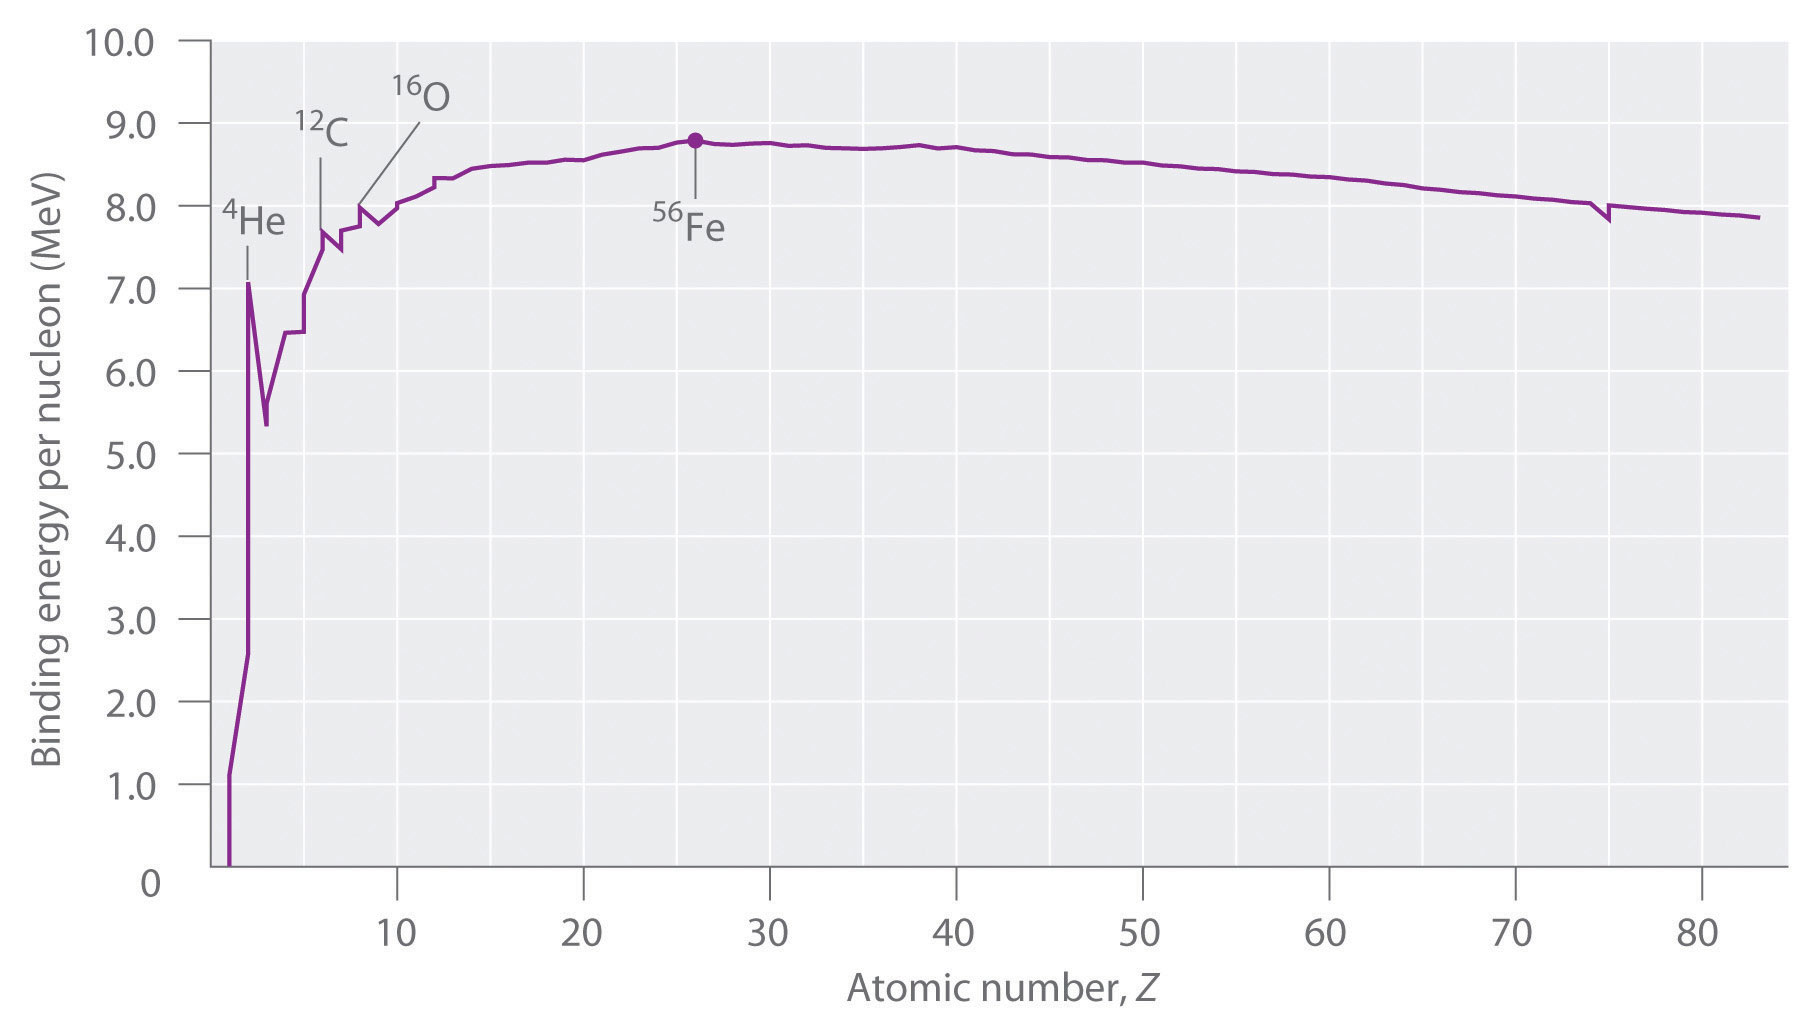
\includegraphics[scale=0.19]{bepn}
\end{center} 

Notice that Iron has the greatest binding energy per nucleon and so is the most
stable isotope in nature. Helium is also anomolously stable, as are Carbon and
Oxygen.

This graph can tell us what nuclear processes each isotope will occur in.
Isotopes with a higher mass than Iron (greater than 56) will participate in
fission and isotopes with a lower mass than Iron (less than 56) will participate
in fusion.

\paragraph*{Fission} occurs when a large nucleus splits into two smaller nuclei.
If the two resulting nucleus' have a greater binding energy than that of the
initial one, then energy will have been released. With regard to Uranium 235, a
neutron is absorbed, and then the nucleus splits into two lighter fragments (and
two or more neutrons).

\paragraph*{Fusion} occurs when two light nuclei fuse together to become one.
The final binding energy per nucleon is greater than the initial value, and
energy will be released. Helium has a larger binding energy per nucleon than
Lithium, so it actually absorbs energy when it fuses.

\section*{How does fission work in power plants}

In order for fission to occur, a neutron is fired at an unstable nucleus, which
then breaks down into two more nuclei, releasing between two and four more
neutrons as it does so. Since more neutrons are released by this reaction than
are absorbed, a chain reaction occurs, and the rate of reaction (without
intervention) increases exponientially.

The heat from a fission reactor turns water to steam, which turns turbines to generate electricity, as shown below:

\begin{center}
	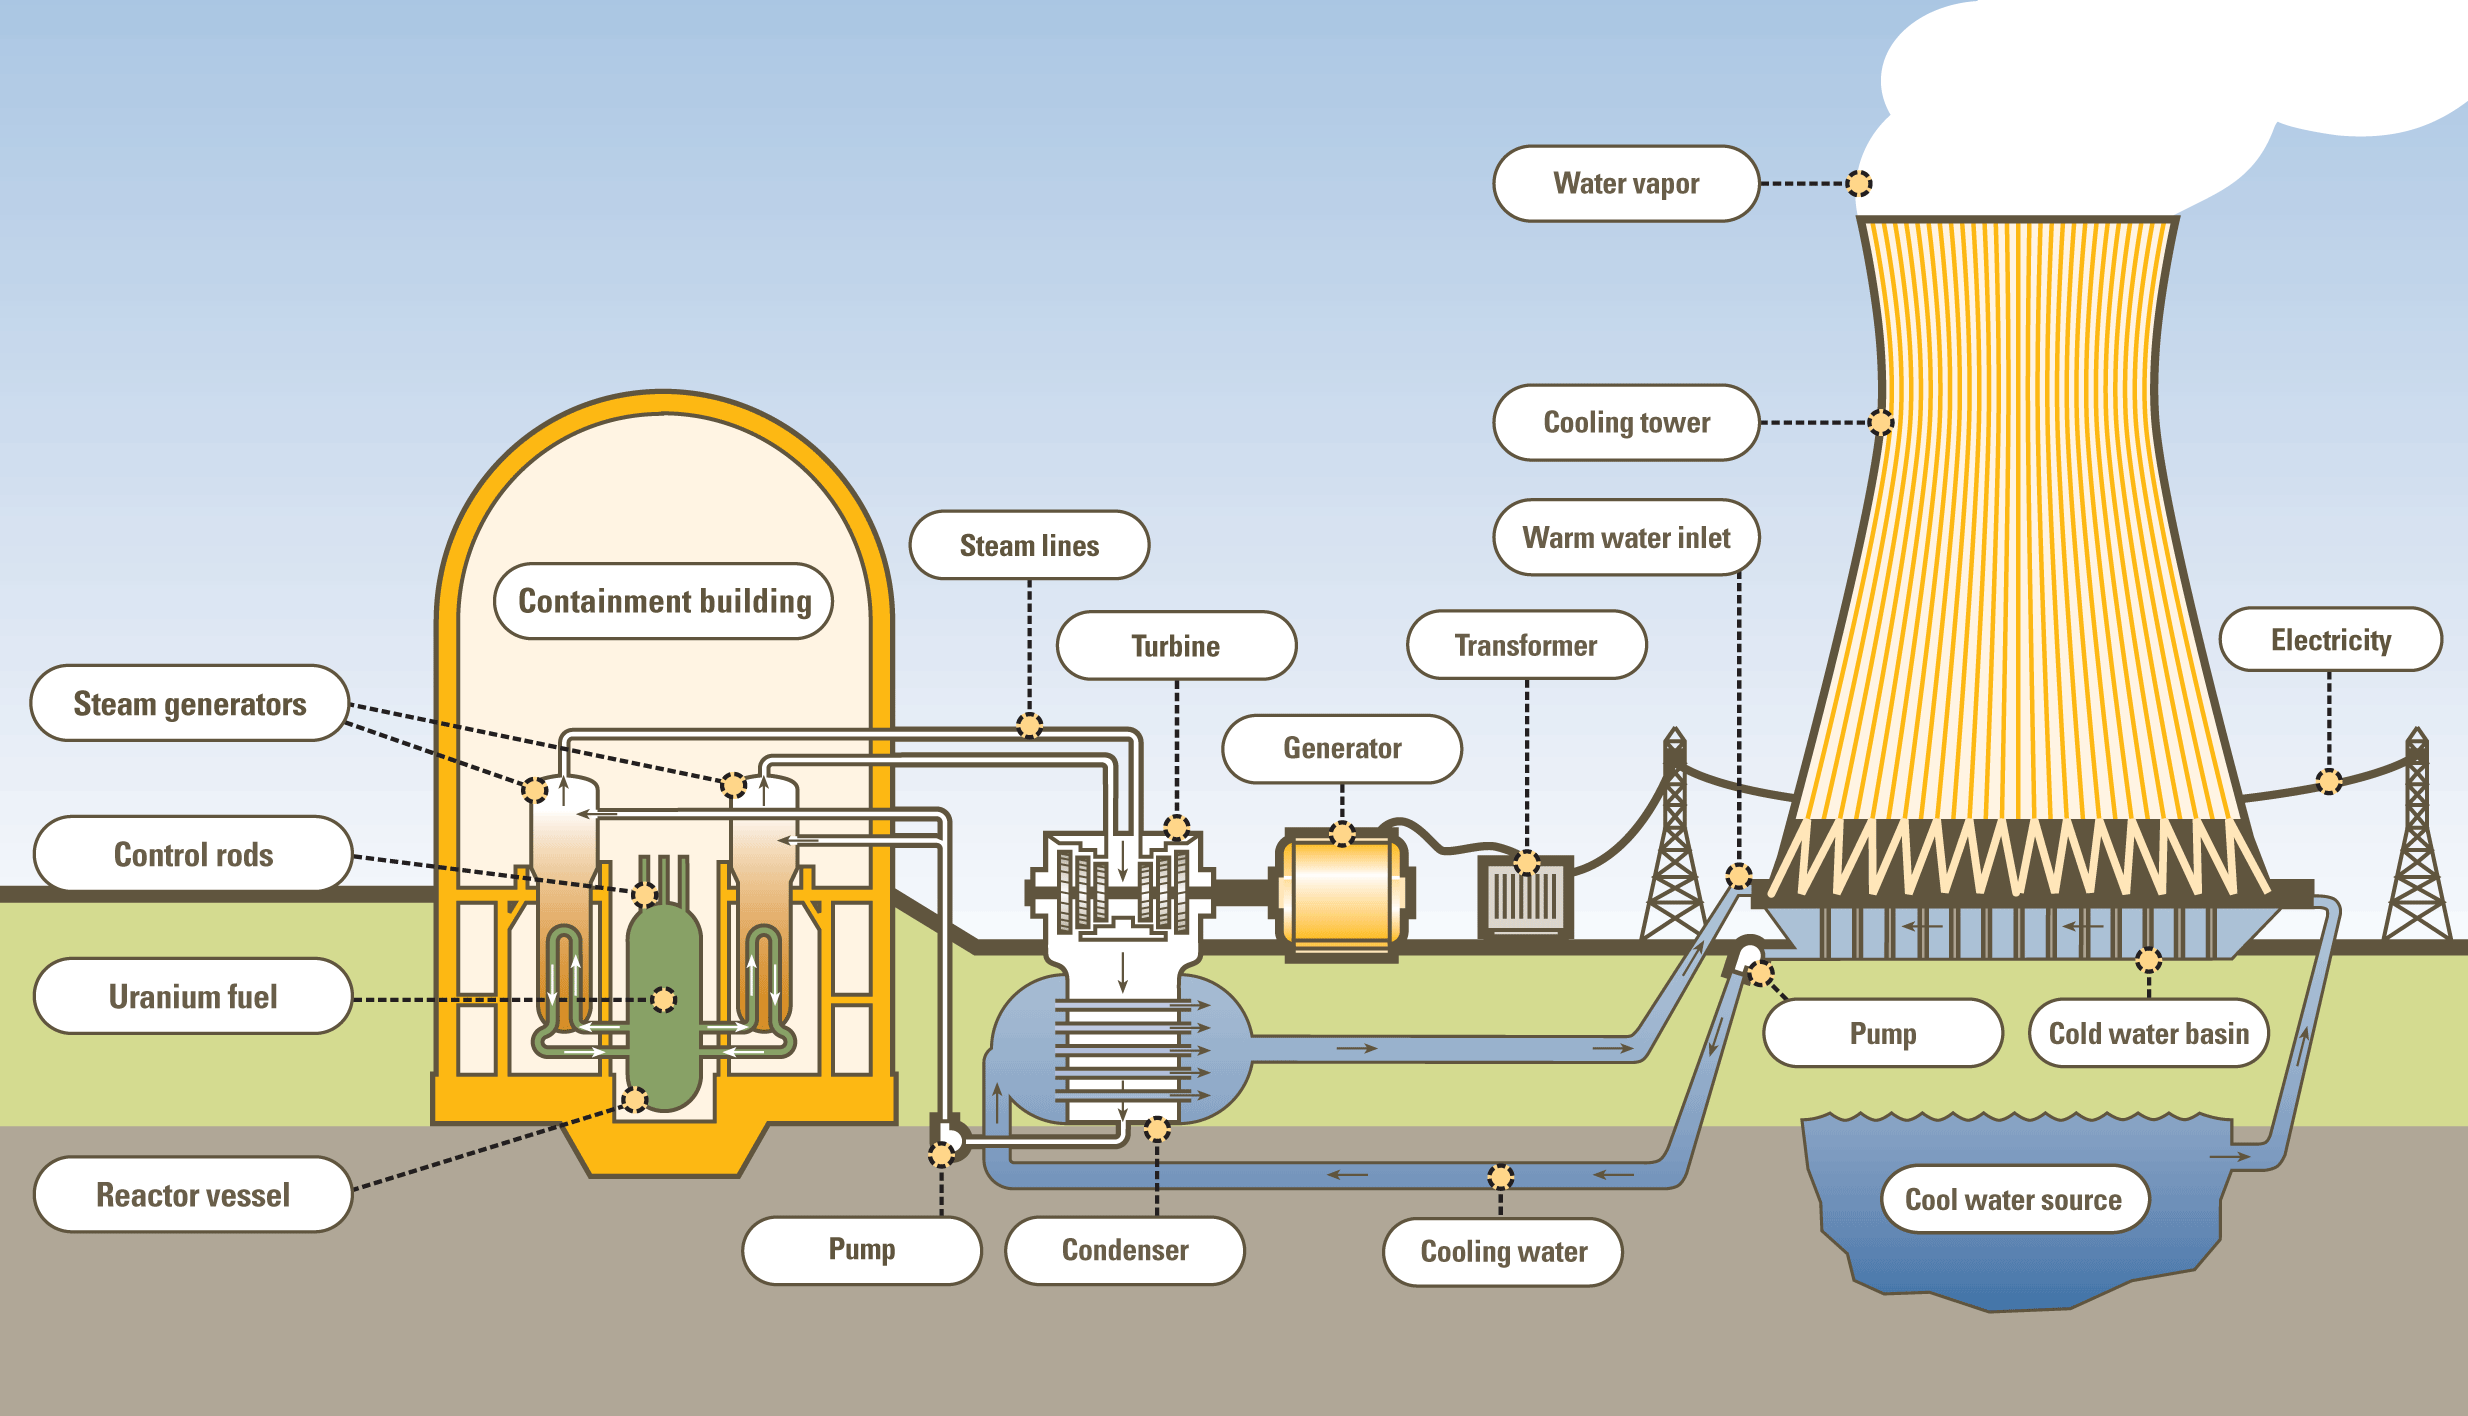
\includegraphics[scale=0.18]{reactor}
\end{center}

Control rods can be moved up and down inside the reactor, moving down inbetween
the radioactive rods to slow the rate of reaction. The control rods are
surrounded by a moderator (that doesn't move up and down with them), that
functions to slow down the neutrons from the radioactive substance before they
hit the control rods. They do this by having inelastic collisions with the
carbon atoms in the moderator. 

Slowing down the neutrons (to around 3\kilo\meter\second$^{-1}$)means that they
are more likley to cause a fission with another uranium nuclei.

The control rods are made of materials such as boron that will absorb the
neutrons in order to slow the reaction if need be.

When a certain percentage of the uranium-235 in the rods has been split, less
than one neutron per fission event reaches another fissile nucleus. This means
that the reaction will gradually slow down.

Once the uranium in the fuel rods has been used up, only the fragments from the
fission reaction are left. Depending on the fuel used, these products could
decay rapidly (and require cooling for many months), or decay more slowly over
thousands of years.

\section*{Questions}

\subsection*{Question 1}

If all of the nuclei in 1.0\kilo\gram of uranium-235 undergo fission, it's mass
decreases by 0.90\gram. {\bf a)} Find the energy released. {\bf b)} If somebody
uses energy at an average rate of 1\kilo\watt, estimate how much uranium would
be used over their life.

\subsection*{Answer 1}

\paragraph{a)}
\setlength\parindent{20pt}

$E=mc^2$

$E = 0.9\times10^{-3} \times (3\times10^8)^2$

$E = 8.1\times10^{13}\joule$

\paragraph*{b)}
\setlength\parindent{20pt}

1\kilo\watt = 1000\joule\second$^{-1}$

Number of seconds in life = 80 $\times$ 365.25 $\times$ 24 $\times$  60 $\times$ 60 = 2524608000\second

Total energy comsumption = 1000 $\times$ 2524608000 = 2524608000000\joule

Mass of uranium used = $2524608000000 \div 8.1\times10^{13} = 0.031\kilo\gram$

\subsection*{Question 2}
\setlength\parindent{0pt}

The sun has a power output of around $4.0\times10^{26}$\watt. Estimate the
decrease in the mass of the sun every second.

\subsection*{Answer 2}

\begin{tabular}{p{0.45\textwidth} | p{0.5\textwidth}}

$E=mc^2$ & $m = \frac{4.0\times10^{26}}{(3\times10^8)^2}$\\

$4.0\times10^{26}=m\times(3\times10^8)^2$ & $m = 4.4\times10^9\kilo\gram$\\

\end{tabular}

\end{document}